\documentclass[12pt]{report}
\usepackage[spanish]{babel}
\usepackage[utf8]{inputenc}
\usepackage{amsmath}
\usepackage{amssymb}
\usepackage{amsthm}
\usepackage[mathscr]{euscript}
\usepackage{graphics}
\usepackage{wrapfig}
\usepackage{subfigure}
\usepackage{lipsum}
\usepackage{array}
\usepackage{multicol}
\usepackage{enumerate}
\usepackage[framemethod=TikZ]{mdframed}
\usepackage[a4paper, margin = 1.5cm]{geometry}
\usepackage{bbm}

%En esta parte se hacen redefiniciones de algunos comandos para que resulte agradable el verlos%

\renewcommand{\theenumii}{\roman{enumii}}

\def\proof{\paragraph{Demostración:\\}}
\def\endproof{\hfill$\blacksquare$}

\def\sol{\paragraph{Solución:\\}}
\def\endsol{\hfill$\square$}

%En esta parte se definen los comandos a usar dentro del documento para enlistar%

\newtheoremstyle{largebreak}
  {}% use the default space above
  {}% use the default space below
  {\normalfont}% body font
  {}% indent (0pt)
  {\bfseries}% header font
  {}% punctuation
  {\newline}% break after header
  {}% header spec

\theoremstyle{largebreak}

\newmdtheoremenv[
    leftmargin=0em,
    rightmargin=0em,
    innertopmargin=-2pt,
    innerbottommargin=8pt,
    hidealllines = true,
    roundcorner = 5pt,
    backgroundcolor = gray!60!red!30
]{exa}{Ejemplo}[section]

\newmdtheoremenv[
    leftmargin=0em,
    rightmargin=0em,
    innertopmargin=-2pt,
    innerbottommargin=8pt,
    hidealllines = true,
    roundcorner = 5pt,
    backgroundcolor = gray!50!blue!30
]{obs}{Observación}[section]

\newmdtheoremenv[
    leftmargin=0em,
    rightmargin=0em,
    innertopmargin=-2pt,
    innerbottommargin=8pt,
    rightline = false,
    leftline = false
]{theor}{Teorema}[section]

\newmdtheoremenv[
    leftmargin=0em,
    rightmargin=0em,
    innertopmargin=-2pt,
    innerbottommargin=8pt,
    rightline = false,
    leftline = false
]{propo}{Proposición}[section]

\newmdtheoremenv[
    leftmargin=0em,
    rightmargin=0em,
    innertopmargin=-2pt,
    innerbottommargin=8pt,
    rightline = false,
    leftline = false
]{cor}{Corolario}[section]

\newmdtheoremenv[
    leftmargin=0em,
    rightmargin=0em,
    innertopmargin=-2pt,
    innerbottommargin=8pt,
    rightline = false,
    leftline = false
]{lema}{Lema}[section]

\newmdtheoremenv[
    leftmargin=0em,
    rightmargin=0em,
    innertopmargin=-2pt,
    innerbottommargin=8pt,
    roundcorner=5pt,
    backgroundcolor = gray!30,
    hidealllines = true
]{mydef}{Definición}[section]

\newmdtheoremenv[
    leftmargin=0em,
    rightmargin=0em,
    innertopmargin=-2pt,
    innerbottommargin=8pt,
    roundcorner=5pt
]{excer}{Ejercicio}[section]

%En esta parte se colocan comandos que definen la forma en la que se van a escribir ciertas funciones%

\newcommand\abs[1]{\ensuremath{\left|#1\right|}}
\newcommand\divides{\ensuremath{\bigm|}}
\newcommand\cf[3]{\ensuremath{#1:#2\rightarrow#3}}
\newcommand\natint[1]{\ensuremath{\left[\!\left[ #1\right]\!\right]}}
\newcommand{\afa}{\:
    \begin{tikzpicture}
        \draw [line width = 0.17 mm, black] (0,0) -- (-0.115,0.29);
        \draw [line width = 0.17 mm, black] (0,0) -- (0.115,0.29);
        \draw [line width = 0.17 mm, black] (-0.12,0) arc (190:-10:0.12cm);
    \end{tikzpicture}
    \:
}
%Este símvolo es para casi todo salvo una cantidad finita

%recuerda usar \clearpage para hacer un salto de página

\begin{document}
    \setlength{\parskip}{5pt} % Añade 5 puntos de espacio entre párrafos
    \setlength{\parindent}{12pt} % Pone la sangría como me gusta
    \title{Notas Taller Topología Algebraica}
    \author{Cristo Daniel Alvarado}
    \maketitle

    \tableofcontents %Con este comando se genera el índice general del libro%

    \setcounter{chapter}{1} %En esta parte lo que se hace es cambiar la enumeración del capítulo%
    
    \chapter{Grupos Libres y Productos de Grupos Libres}
    
    En los capítulos siguientes será indispensable el tratar con este tipo de grupos dada la naturaleza del grupo fundamental de los espacios topológicos.
    
    \section{Producto Débil de Grupos}
    
    \begin{obs}
        De ahora en adelante, el símbolo $\afa$ significa \textit{para casi todo salvo una cantidad finita de elementos}.
    \end{obs}

    \begin{obs}
        En esta parte, $I$ no denotará al intervalo $[0,1]$, sino a una indexación de una familia.
    \end{obs}

    \begin{mydef}
        Sea $\mathcal{G}=\left\{G_i \right\}_{ i\in I}$ una familia arbitraria no vacía de grupos. Se define el \textbf{producto directo de la familia $\mathcal{G}$} por:
        \begin{equation*}
            \prod\mathcal{G}=\left\{\cf{x}{I}{\prod_{ i\in I}G_i}\Big|x\textup{ es función} \right\}
        \end{equation*}
        y en ocasiones se denotará simplemente por $\prod_{ i\in I}G_i$. Se dota a este conjunto de la siguiente operación: si $x,y\in\prod\mathcal{G}$, entonces $\cf{x\cdot y}{I}{\prod_{ i\in I}G_i}$ es la función tal que
        \begin{equation*}
            (x\cdot y)(i)=x(i)\cdot y(i)
        \end{equation*}
        para todo $i\in I$, siendo la multiplicación respectiva en cada grupo.
    \end{mydef}

    En caso de que no lo haya hecho, queda como ejercicio al lector probar que el producto directo de una familia de grupos $\mathcal{G}$ es un grupo dotado de la operación de la definición anterior.

    \begin{mydef}
        Sea $\mathcal{G}=\left\{G_i \right\}_{ i\in I}$ una familia arbitraria no vacía de grupos. Se define el \textbf{producto débil de la familia $\mathcal{G}$} como el subgrupo de $\prod\mathcal{G}$ dado por:
        \begin{equation*}
            \prod\mathcal{G}^*=\left\{x\in\prod\mathcal{G}\Big|x(i)=e_i,\afa i\in I \right\}
        \end{equation*}
        donde $e_i$ denota la identidad de $G_i$ para cada $i\in I$.
    \end{mydef}

    \begin{propo}
        Si $\mathcal{G}$ es una familia arbitraria no vacía de grupos, entonces
        \begin{equation*}
            \prod\mathcal{G}^*<\prod\mathcal{G}
        \end{equation*}
        es decir, que $\prod\mathcal{G}^*$ es un subgrupo de $\prod\mathcal{G}$.
    \end{propo}

    \begin{proof}
        Ejercicio.
    \end{proof}

    \begin{mydef}
        Sea $\mathcal{G}=\left\{G_i \right\}_{ i\in I}$ una familia no vacía de grupos. Si $G_i$ es abeliano para cada $i\in I$, entonces llamaremos a $\prod\mathcal{G}^*$ la \textbf{suma directa de los grupos $G_i$}. En este caso, se denotará la operación del grupo de forma aditiva y se le denotará por:
        \begin{equation*}
            \prod\mathcal{G}^*=\bigoplus_{ i\in I}G_i=\bigoplus\mathcal{G}
        \end{equation*}
    \end{mydef}

    \begin{obs}
        Note que ambas definiciones coinciden si $I$ es un conjunto finito.
    \end{obs}

    \begin{mydef}
        En las condiciones de la definición anterior, para cada índice $i\in I$ definimos un \textbf{monomorfismo natural} $\cf{\varphi_i}{G_i}{\prod\mathcal{G}^*}$ definido como sigue: $\forall g\in G_i$ y para todo $j\in I$:
        \begin{equation*}
            (\varphi_i(g))(j)=\left\{
                \begin{array}{lcr}
                    g & \textup{ si } & i = j\\
                    e_j & \textup{ si } & i\neq j\\
                \end{array}
            \right.
        \end{equation*}
    \end{mydef}

    En el caso en que cada $G_i$ sea un grupo abeliano, el siguiente teorema da una caracterización importante de su producto débil y de los monomorfismos $\varphi_i$.

    \begin{theor}
        Si $\left\{G_i \right\}_{ i\in I}$ es una familia no vacía de grupos abelianos y,
        \begin{equation*}
            G=\bigoplus_{ i\in I}G_i
        \end{equation*}
        
        \begin{center}
            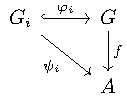
\includegraphics[scale=1.5]{images/fig_1.pdf}
        \end{center}
    \end{theor}

    \section{Generadores y Relaciones}

    \begin{mydef}
        Sea $F$ un grupo y $X\subseteq F$ un grupo, decimos que $F$ es un \textbf{grupo libre con base $X$}, si para cada grupo $G$ y para cada función $\cf{f}{X}{G}$, existe un único homomorfismo $\cf{\varphi}{F}{G}$ extensión de $F$ tales que el diagrama
        
    \end{mydef}

\end{document}